\chaptertoc{Annexes}\markboth{ANNEXES}{}
\setcounter{section}{0}
\renewcommand{\thesection}{\Alph{section}}
\renewcommand{\theHsection}{appendixsection.\Alph{section}}
\section{Cycle de vie d'une activité d'Android }
\begin{figure}[H]
	\centering
	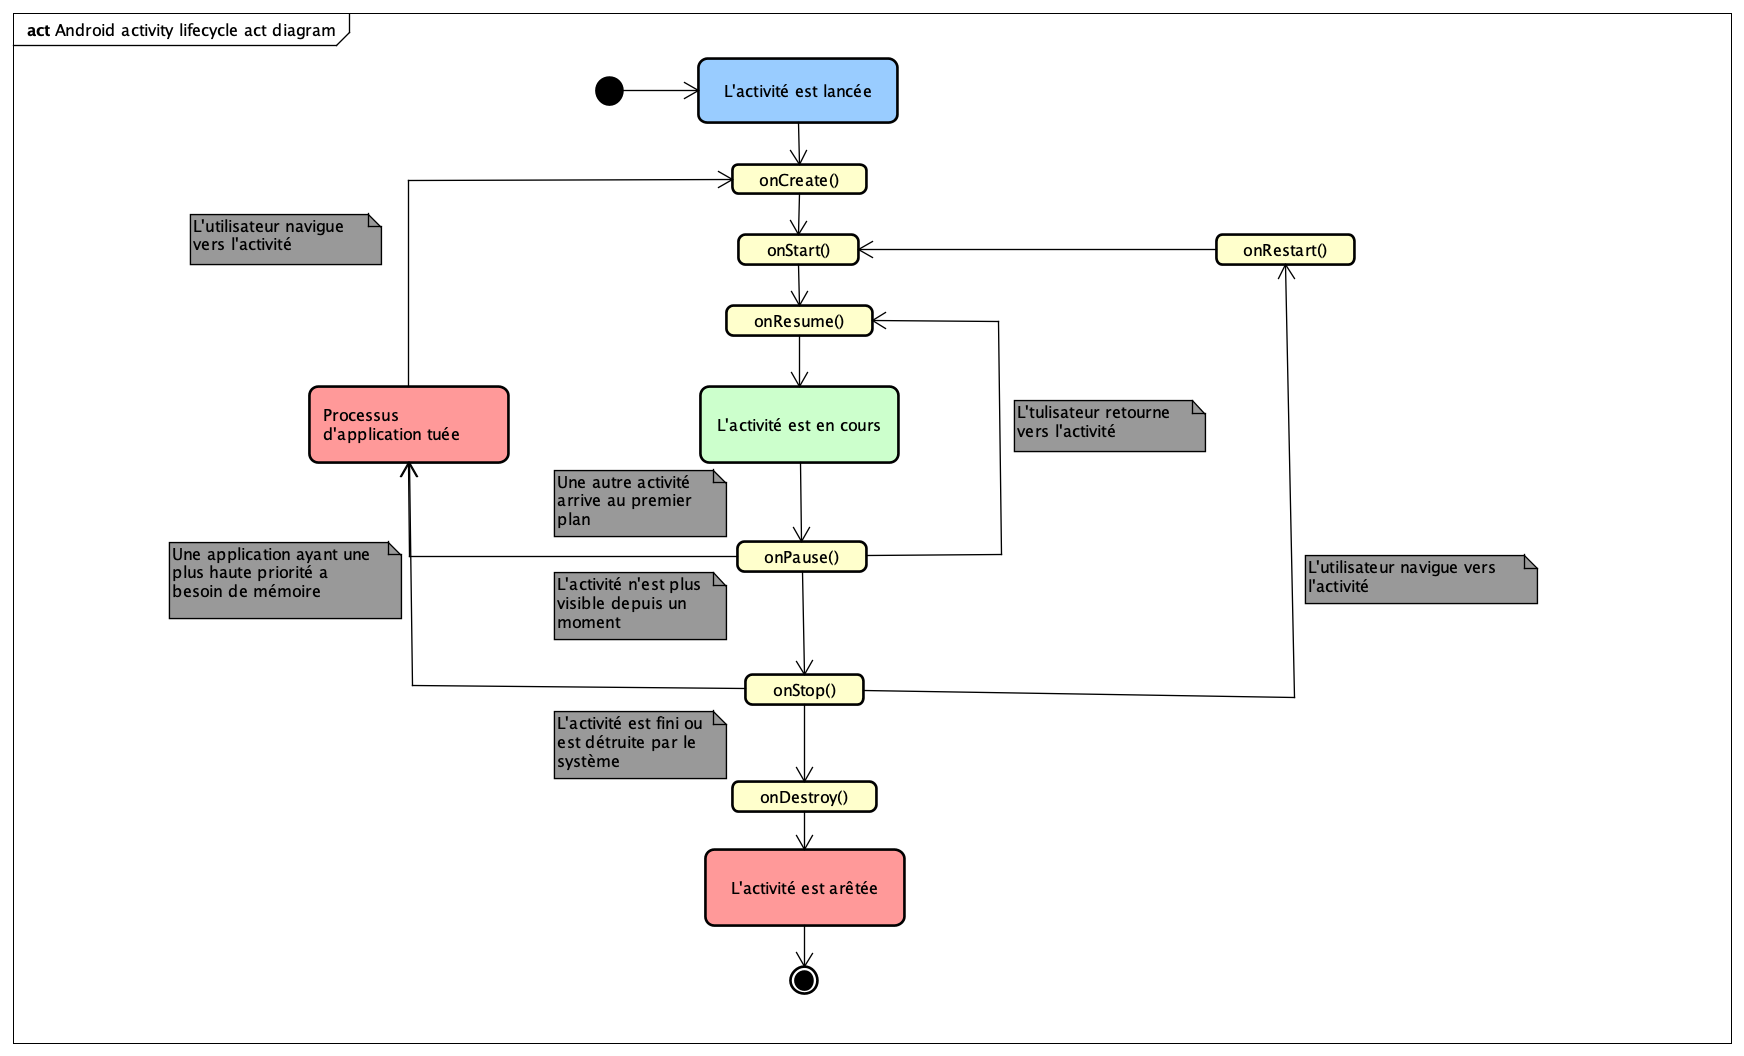
\includegraphics[scale=0.4]{assets/images/Android_lifecycle_act_diagram.png}
	\caption{Diagramme d'activité du cycle de vie d'une activité Android}
	\label{fig.android_act}
\end{figure}
\newpage
\section{Diagramme de séquence du cycle de vie d'une activité}
\begin{figure}[H]
	\centering
	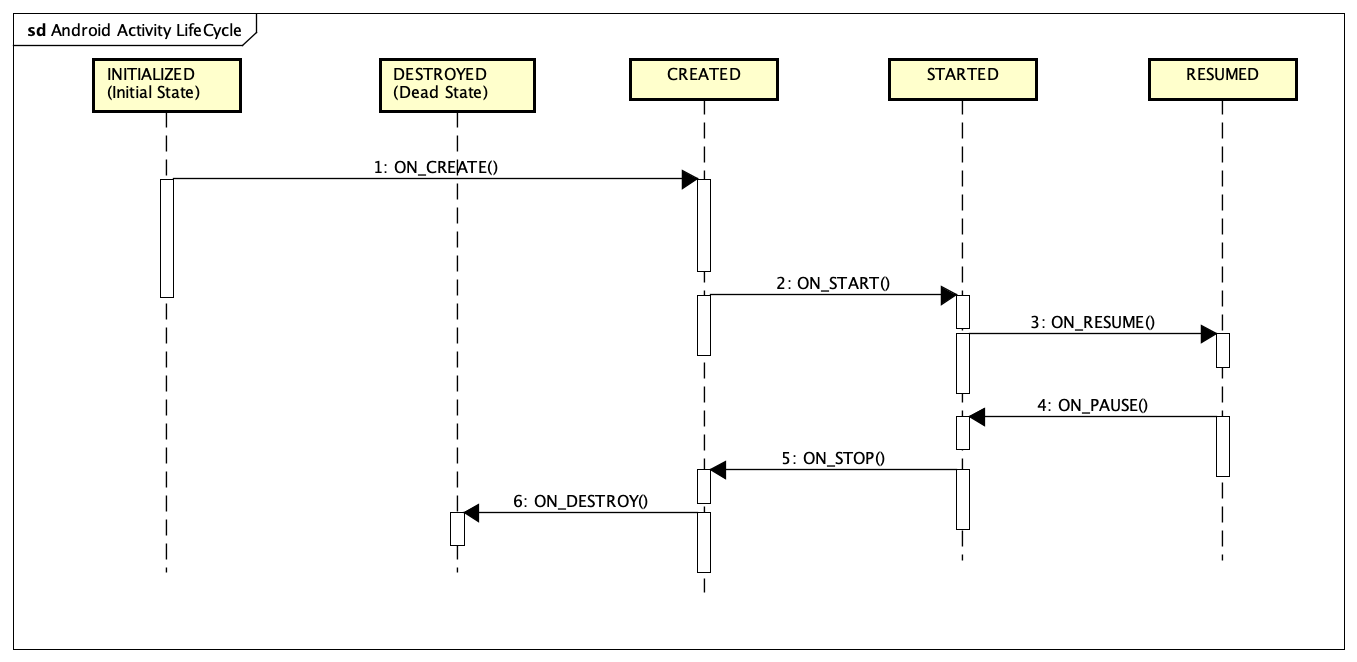
\includegraphics[scale=0.5]{assets/images/Android_LifeCycle_seq.png}
	\caption{Diagramme de séquence du cycle de vie d'une activité Android}
	\label{fig.android_seq}
\end{figure}
\section{Diagramme d'état du cycle de vie d'une activité}
\begin{figure}[H]
	\centering
	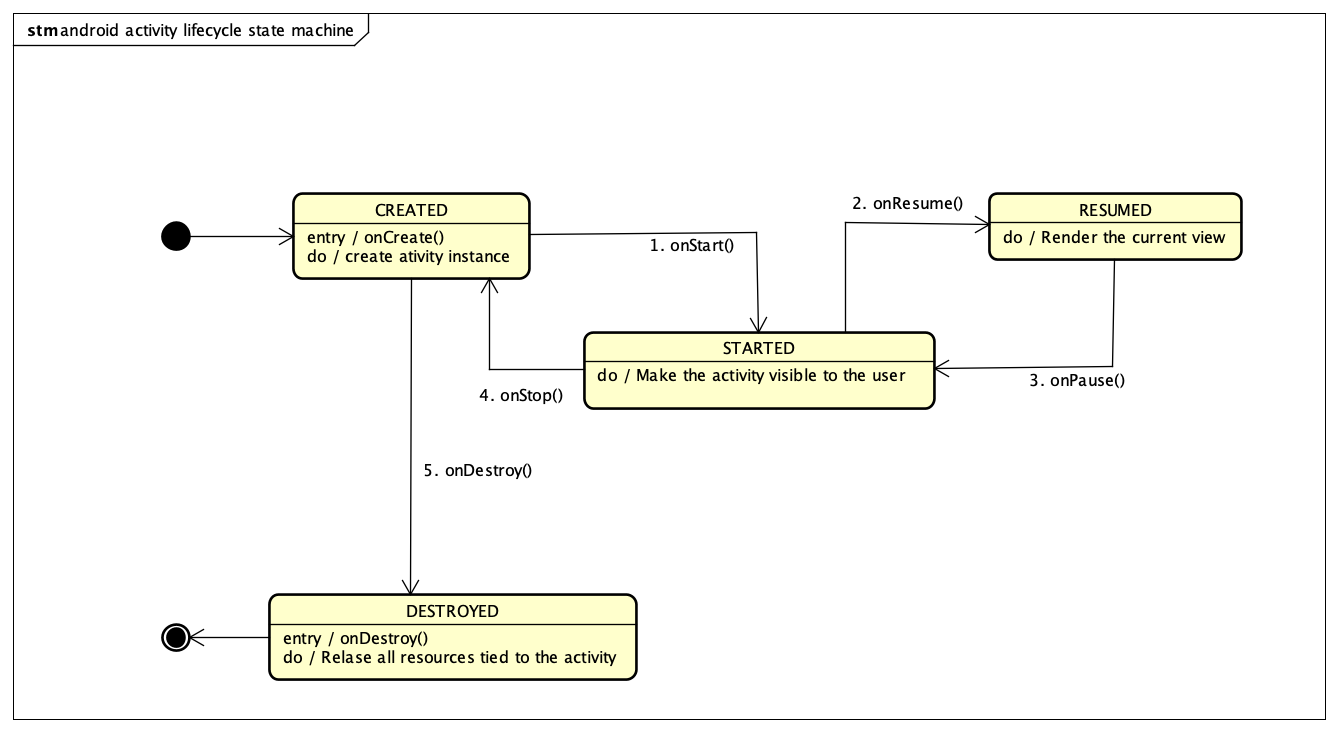
\includegraphics[scale=0.5]{assets/images/android_lifecycle_state_machine.png}
	\caption{Diagramme de état-transition du cycle de vie d'une activité Android}
	\label{fig.android_state}
\end{figure}
\section{Gestion du panier}
\begin{figure}[H]
	\centering
	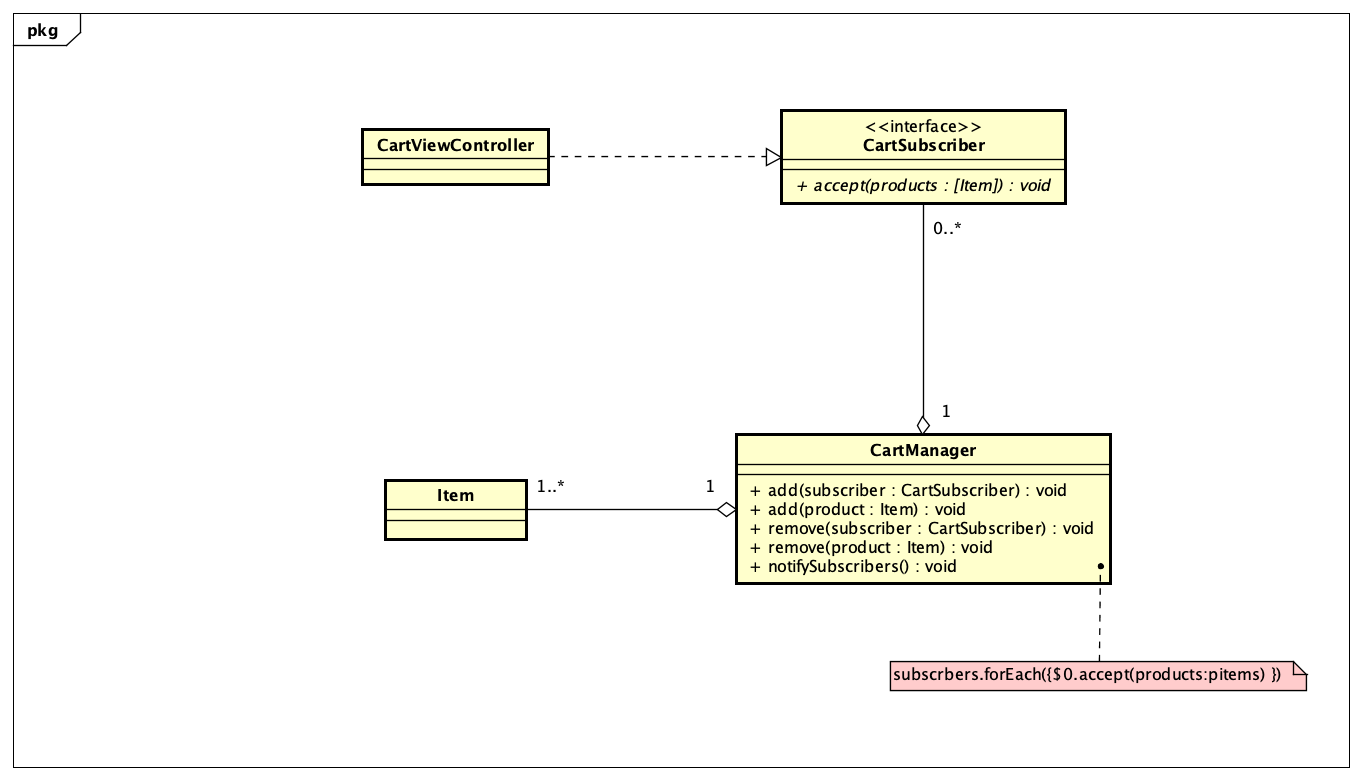
\includegraphics[scale=0.45]{assets/images/cart_management.png}
	\caption{Diagramme de classe de la gestion des paniers}
	\label{fig.android_cart_man}
\end{figure}
\section{Diagramme d'activité du cycle de vie d'une activité iOS}
\begin{figure}[H]
	\centering
	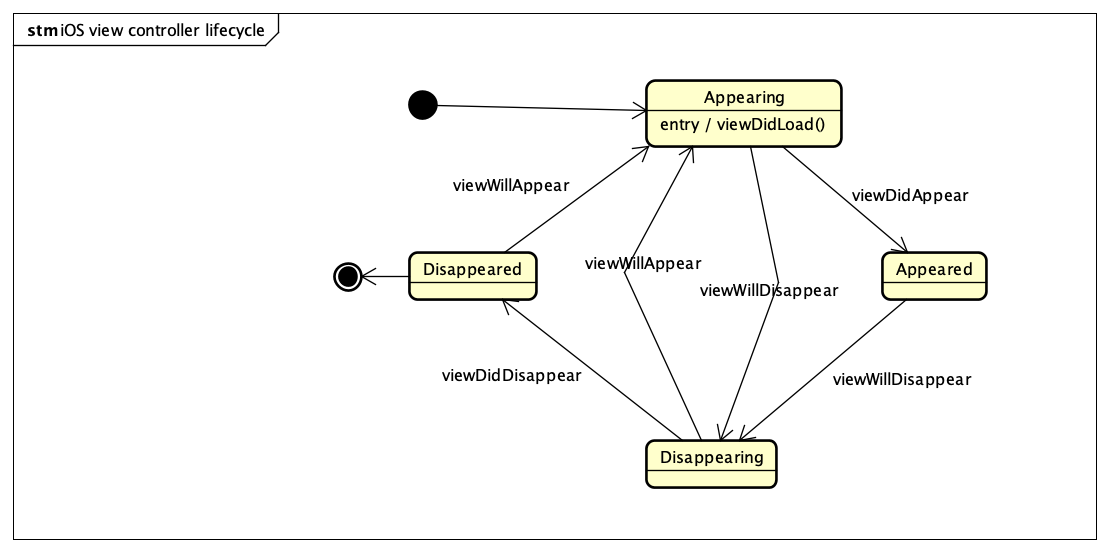
\includegraphics[scale=0.55]{assets/images/iOS_view_lifecycle.png}
	\caption{Diagramme d'activité des cycles de vie}
	\label{fig.ios_act}
\end{figure}
\section{Architecture Viper}
\begin{figure}[H]
	\centering
	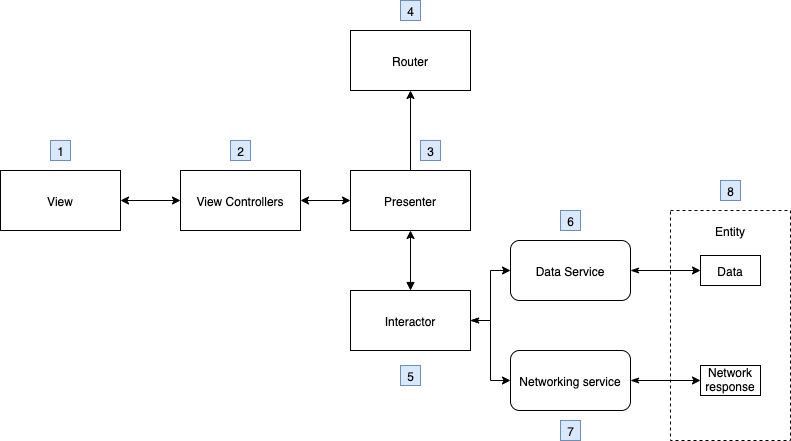
\includegraphics[scale=0.55]{assets/images/viper_one.png}
	\caption{Description de l'architecture VIPER}
	\label{fig.ios_viper}
\end{figure}
\section{Exemple d'application de l'architecture VIPER}
\begin{figure}[H]
	\centering
	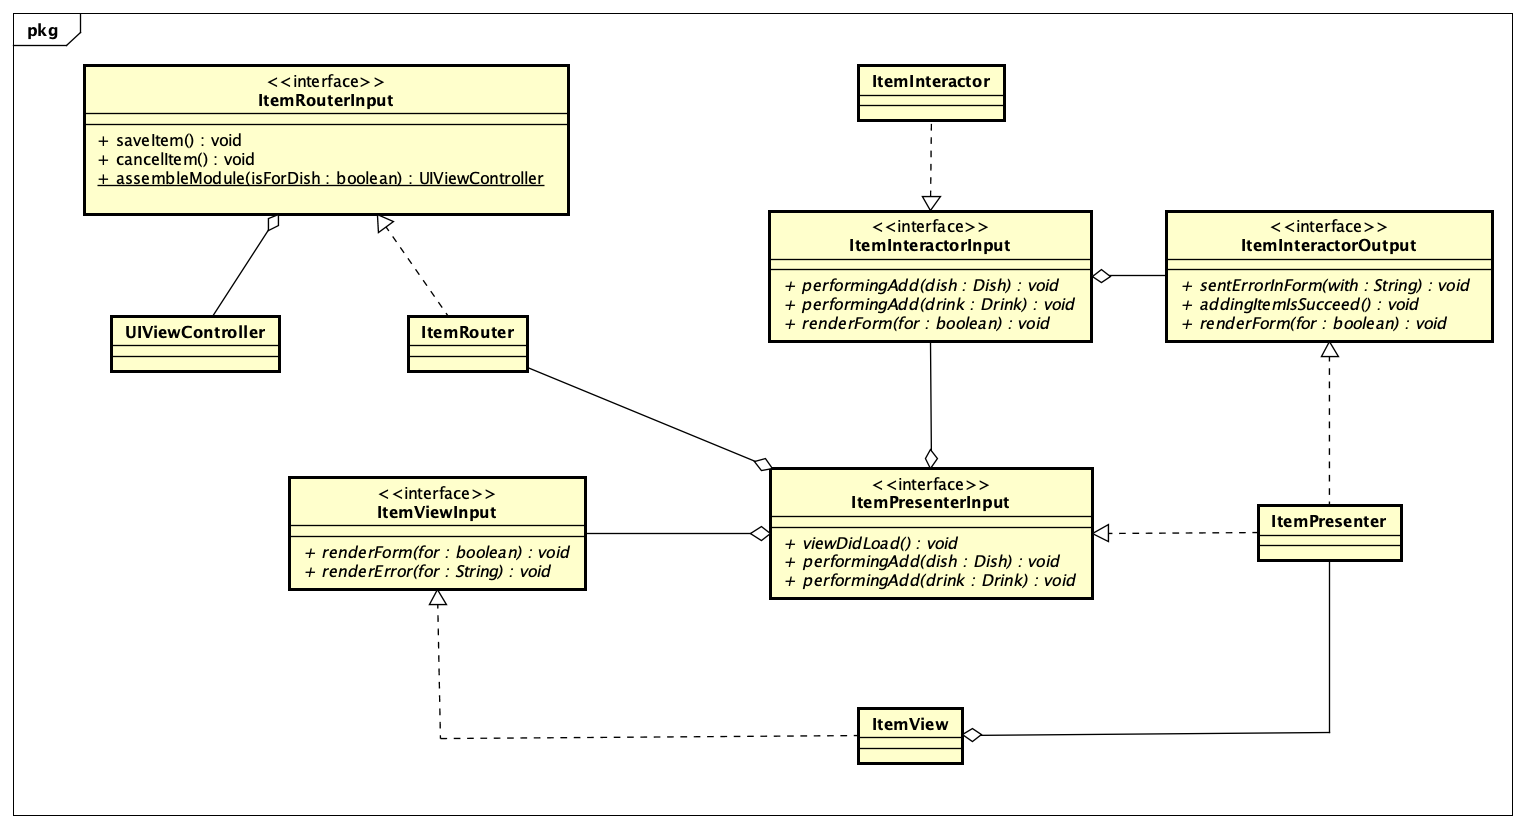
\includegraphics[scale=0.4]{assets/images/viper_example.png}
	\caption{Diagramme de classe d'un composant de l'application avec l'architecture VIPER}
	\label{fig.ios_viper_example}
\end{figure}